%%%%%%%%%%%%%%%%%%%%%%%%%%%%%%%%%%%%%
\section{Base \ttfamily R \normalfont Plots}
%%%%%%%%%%%%%%%%%%%%%%%%%%%%%%%%%%%%%
\subsection{Creating Plots}
% --------------------------------------------------- Slide --
\begin{frame}[ fragile]
  \frametitle{Creating Plots in R}
  \begin{columns}
      \column{0.50\textwidth}
        \begin{itemize}
           \item To make a plot in R, you can use \ttfamily plot(): \normalfont \\
		\begin{lstlisting}
			# Load data
			library(alr3)
			data(UN2)
			attach(UN2)
			# Plot variables
plot(logFertility~logPPgdp, xlab="logPPgdp", ylab="logFertility", 
main="logGDP vs logFertility Plot")
		\end{lstlisting}
         \end{itemize}
%
      \column{0.50\textwidth}
       \begin{center}
         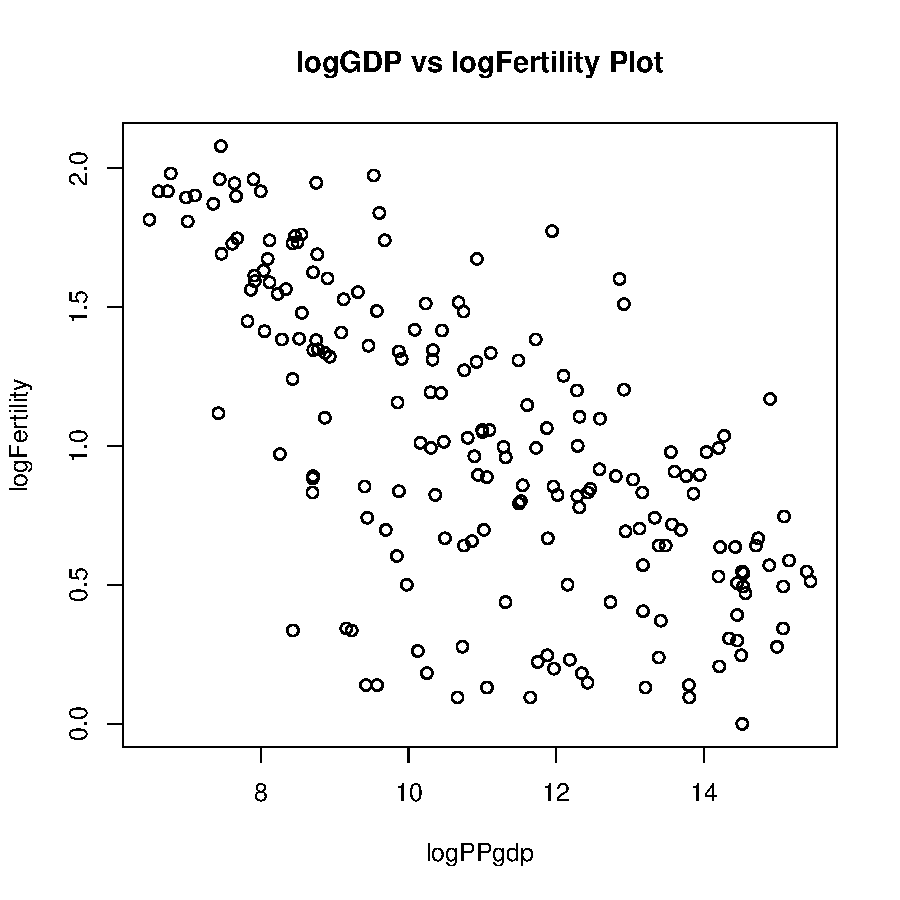
\includegraphics[width=1\textwidth]{images/UN2plot.pdf}
        \end{center}
      \end{columns}
\end{frame}      

\subsection{Adding Details to Plots}
\begin{frame}[fragile, allowframebreaks]
  \frametitle{Adding Details}
  \framesubtitle{Adding Other Variables}
  	      
      		\begin{lstlisting}
			# Step 1: Load the Data
			library(alr3)
			data(UN2); attach(UN2)
			# Step 2: Subset appropriately
			ind<-which(Purban>50)
			# Step 3: Plot		
			plot(logFertility~logPPgdp, xlab="logPPgdp", ylab="logFertility", main="logGDP vs logFertility Plot")
			points(logFertility[ind]~logPPgdp[ind], col="red", pch=19)
			legend("topright", pch=c(1,19), col=1:2, c("Purban<50", "Purban>=50"))
		\end{lstlisting}
%
\newpage
       \begin{center}
         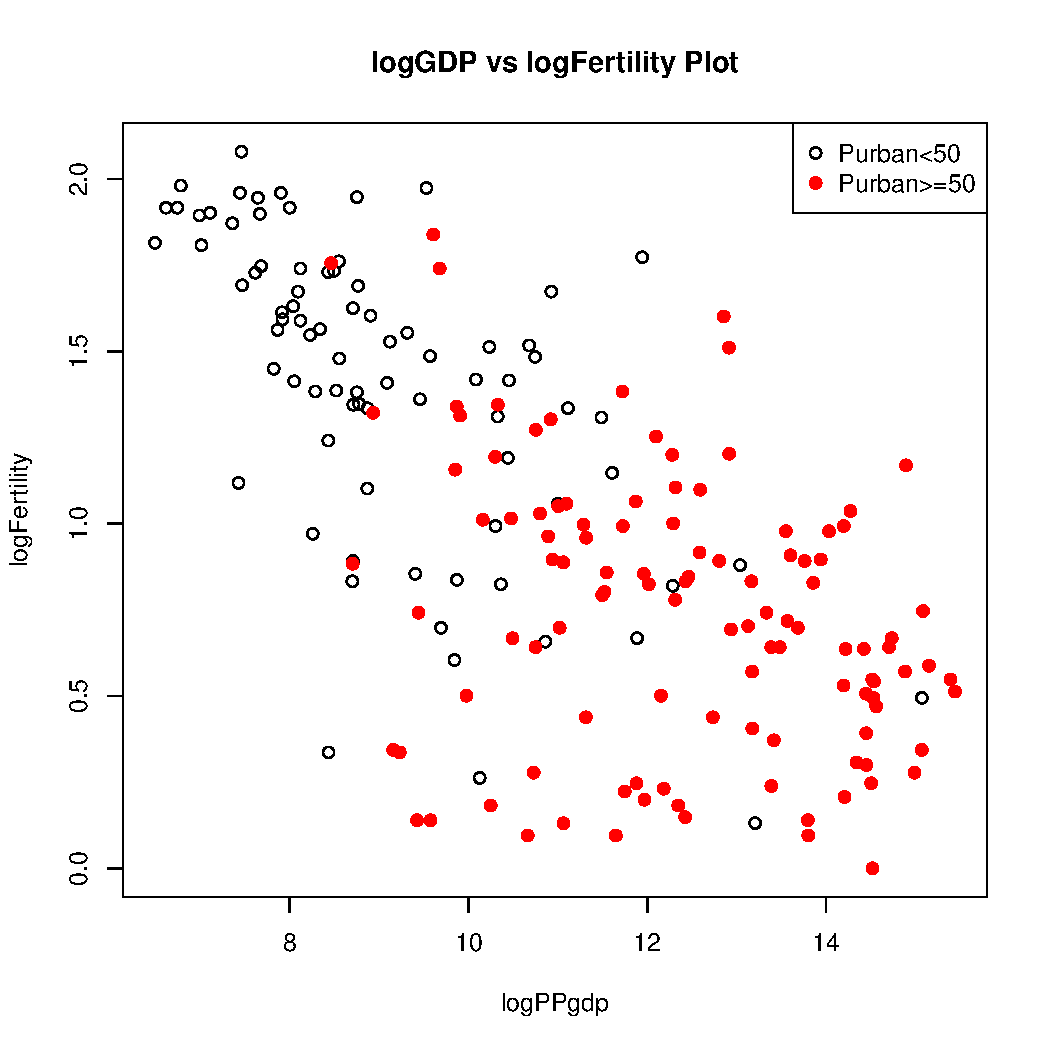
\includegraphics[width=0.65\textwidth]{images/Unplot3.pdf}
        \end{center}

\end{frame}

%%%%%%%%%%%%%%%%%%%%%%%%%%%%%%%%%%%%%
\begin{frame}[fragile, allowframebreaks]
  \frametitle{Adding Details}
  \framesubtitle{Highlighting Observations}
  	      
      		\begin{lstlisting}
# Step 1: Generate Data
set.seed(3012008)
x=rnorm(100)
y=-x+I(x^2) +rnorm(100)
# Step 2: Plot Data
plot(y~x)
# Step 3: Highlight top 10% of observations (according to y)
a=sort(y, decreasing=T)
b=round((length(y))*.1, digits=0); b
points(y[which(y>=a[b])]~x[which(y>=a[b])], col="red")
		\end{lstlisting}
%
\newpage
       \begin{center}
         \includegraphics[width=0.65\textwidth]{images/top10.png}
        \end{center}

\end{frame}


%%%%%%%%%%%%%%%%%%%%%%%%%%%%%%%%%%%%%
\begin{frame}[fragile, allowframebreaks]
  \frametitle{Adding Details}
  \framesubtitle{Comparing Means}
	      
      		\begin{lstlisting}
data(iris)
attach(iris)
a<-aggregate(iris[, -5], list(Species=Species), mean)
row.names(a)<-a[, 1]
dotchart(t(a[, -1]), xlim=c(0, 10), main="Plots of Means for Iris Data Set", xlab="Mean Value")
		\end{lstlisting}
%
\newpage
       \begin{center}
         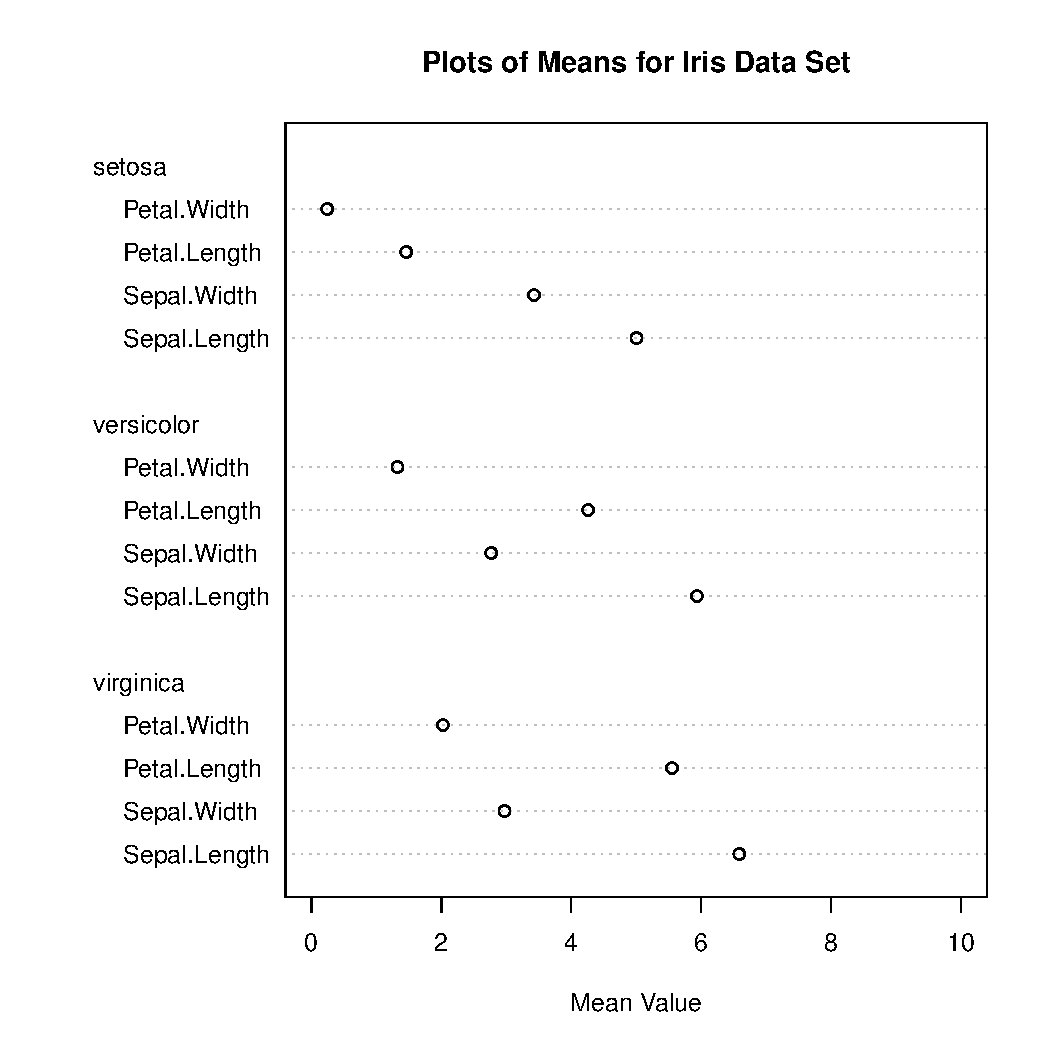
\includegraphics[width=0.65\textwidth]{images/aggPlot.pdf}
        \end{center}

\end{frame}